% Pipeline figure (TikZ, explicit grid in cm). Orange = our additions or changes to the reference recipe.
\begin{tikzpicture}[
    font=\scriptsize, >={Stealth[length=4pt]},
    box/.style={draw=black!55, rounded corners=2pt, fill=base, align=flush center, inner sep=2.5pt, line width=0.4pt},
    ours/.style={box, draw=oursline, fill=oursfill, line width=0.6pt},
    lbl/.style={align=flush center, inner sep=1pt, text=black!75},
    arr/.style={->, line width=0.5pt, draw=black!70},
  ]
  % input, preprocessing, augmentation
  \node[inner sep=0pt] (in) at (0.8, 0.1) {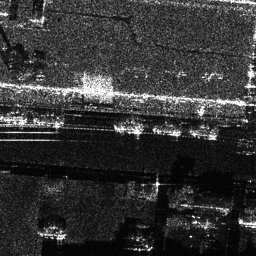
\includegraphics[width=1.5cm]{figs/thumb_input.png}};
  \node[lbl, below=0.4mm of in] {SAR image\\(gray, $\le$\,512 px)};
  \node[box, text width=1.5cm] (pre) at (2.78, 0.1) {resize 512$^2$,\\SAR mean/std,\\gray as RGB};
  \node[ours, text width=3.45cm] (aug) at (1.95, 1.72)
    {\textbf{SAR photometric augmentation}\\speckle $x\sqrt{G}$, $G{\sim}\Gamma(L,\tfrac1L)$, $L{\in}[4,16]$\\gamma $x^{\gamma}$, $\gamma{\in}[\tfrac23,\tfrac32]$ (log-uniform)\\each with $p{=}0.8$ (training only)};
  \draw[arr] (in) -- (pre);
  \draw[arr, draw=oursline] (aug.south -| pre.north) -- (pre.north);
  % shared trunk
  \node[box, minimum width=3.15cm, minimum height=2.5cm] (trunk) at (5.55, 0.2) {};
  \node[lbl, anchor=north, text=black] at (trunk.north) {\textbf{Shared trunk}: YOLO26-L\\backbone + neck};
  \node[lbl, anchor=south] at (trunk.south) {COCO-pretrained,\\26.19\,M params, all trained};
  \foreach \x/\s/\t in {4.62/0.72/{P3 (stride 8)}, 5.52/0.52/{P4 (16)}, 6.32/0.36/{P5 (32)}} {
    \node[draw=black!50, fill=white, minimum width=\s cm, minimum height=\s cm, inner sep=0pt] (f) at (\x, 0.25) {};
    \node[lbl, font=\tiny] at (\x, -0.32) {\t};
  }
  \draw[arr] (pre) -- (pre -| trunk.west);
  % heads
  \node[ours, text width=2.6cm] (cls) at (8.95, 0.82)
    {\textbf{Classification head}\\GAP(P5), LN, Linear\\$z\in\mathbb{R}^9$ (5.6\,k params)};
  \node[box, text width=2.6cm] (det) at (8.95, -0.62)
    {\textbf{Detection heads}\\one-to-many, one-to-one\\boxes $b_n$, scores $s_{n,c}$};
  \draw[arr] (trunk.east |- cls.west) -- (cls.west);
  \draw[arr] (trunk.east |- det.west) -- (det.west);
  % cross-task decoding
  \node[ours, text width=3.25cm] (fuse) at (12.55, 0.86)
    {\textbf{Detector $\to$ class} (ours)\\$\hat z_c=\log\mathrm{softmax}(z)_c$\\$\qquad+\,\beta\log\max_n s_{n,c}$};
  \node[ours, text width=3.25cm] (jd) at (12.55, -0.66)
    {\textbf{Class $\to$ detector} (ours)\\$s'_{n,c}=s_{n,c}\,\hat p_c^{\,\alpha}$, $\hat p=\mathrm{softmax}(\hat z)$\\per-class NMS 0.8, top 100};
  \draw[arr] (cls.east) -- (cls.east -| fuse.west);
  \draw[arr] (det.east) -- (det.east -| jd.west);
  \draw[arr, draw=oursline] (det.north east) -- node[lbl, left=-1pt, font=\tiny, text=oursline, pos=0.55] {$s$}
    (fuse.south west);
  \draw[arr, draw=oursline] ($(fuse.south)+(1.0,0)$) -- node[lbl, right=0pt, font=\tiny, text=oursline] {$\hat p$}
    ($(jd.north)+(1.0,0)$);
  % output
  \node[inner sep=0pt] (out) at (15.4, 0.1) {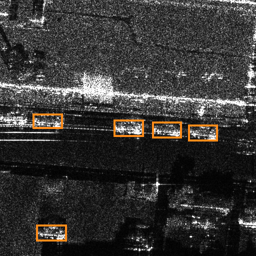
\includegraphics[width=1.5cm]{figs/thumb_output.png}};
  \node[lbl, below=0.4mm of out] {class $\arg\max\hat z$\\+ boxes (one pass)};
  \draw[arr] (fuse.east) -- (out.north west);
  \draw[arr] (jd.east) -- (out.south west);
  % training
  \node[box, fill=white, text width=11.0cm] (train) at (5.75, -2.02)
    {\textbf{Training}: $\mathcal{L}=\mathrm{CE}(z,y)+\mathcal{L}_\text{det}$ (YOLO26 box + class losses on both heads);
     h/v flips; AdamW, lr $5{\times}10^{-4}$, batch 16, cosine, EMA 0.9998, bf16, 350 epochs on all 9{,}392 train images};
  \node[ours, text width=3.95cm] (swa) at (14.0, -2.02)
    {\textbf{SWA} (ours): 12 more epochs at\\lr $5{\times}10^{-5}$, average of the\\12 epoch-end weights};
  \draw[arr] (train) -- (swa);
  % legend
  \node[ours, minimum width=3mm, minimum height=2mm, inner sep=0pt] (lg) at (0.3, -2.72) {};
  \node[lbl, anchor=west] at (0.5, -2.72) {our additions or changes};
  \node[box, minimum width=3mm, minimum height=2mm, inner sep=0pt] (lg2) at (3.25, -2.72) {};
  \node[lbl, anchor=west] at (3.45, -2.72) {standard components};
\end{tikzpicture}
